\pdfoutput=1
\documentclass{l4proj}
\usepackage{amsmath}
\usepackage{subfigure}
\usepackage{caption}
\usepackage{pdfpages}


\begin{document}
\title{Bell-Ringing App for Android}
\author{Allan Macmillan}
\date{March 28, 2014}
\maketitle

\begin{abstract}
The project focusses on creating an Android of application which will be a port of the iOS application MOBEL. MOBEL is an application that bell-ringers can use in order to practice ringing methods. Bell-ringers are able to choose from a number of possible stages, compositions and methods as well as other customisable options in order to vary their bell-ringing experience.  
\end{abstract}

\educationalconsent
%
%NOTE: if you include the educationalconsent (above) and your project is graded an A then
%      it may be entered in the CS Hall of Fame
%
\tableofcontents
%==============================================================================

\chapter{Introduction}
\pagenumbering{arabic}

\section{Problem Overview and Background}
Advancements in technology have made mobile applications part of everyday life, relying on them to perform what would now be considered everyday tasks.  Even now, activities that were performed hundreds of years ago can now be performed on a mobile device.  Bell-ringing, or the style more formally known as change ringing, is an art-form that dates back over 400 years\footnote{http://www.nagcr.org/pamphlet.html}.  Tuned bells are swung in a specific order to create what is known as a method, due to the constraints imposed by physics, no actual melody is rung but rather an ever changing series of notes.

Due to the popularity of bell ringing across the world, a number of applications have been created allowing users to practice their bell ringing talents. These applications have come in many forms and on many platform and one such mobile application, MOBEL, was been designed for iOS. This project is required to create an Android version of the application that will emulate it where possible, and make improvements on its weaknesses.  

With bell-ringing being an activity that has been enjoyed throughout the generations, a number of traditions have been passed down and one such tradition states that a bell-ringer is not permitted to have the method changes during ringing and that they must be committed to memory.  This is the premise for MOBEL's existence,  allowing ringers to practice certain methods in order that they reach a stage where they become so competent that seeing the method changes is no longer a problem.  

\section{Background To Bell-Ringing}
To understand the application, there is a substantial amount of terminology and some governing rules that must first be understood.  MOBEL was mainly designed for those whose interests already lay in bell-ringing and assumptions were made in the original application that users would understand the technical jargon.  

\subsection{Terminology}
\textbf{Method} : A \textit{Method }is a series of instructions, or changes, that instructs the bell-ringers as to which order the bells should be rung in.  A Method can be thought of as the “tune” that is being rung.

\textbf{Rows (Changes)} : A row is completed when every ringer has rung their bell once.  The order in which each bell-ringer will ring their bell is altered to give a different series of notes which are called \textit{Rows} or \textit{Changes}.

\textbf{Stage} : The \textit{Stage} is a reference to the number of bells that will be rung in that particular method.  For example, the stage “Minimus” refers to a 4 bell method and “Major” refers to an 8 bell method.  A complete list of the Stages can be found in Appendix C.

%%%%%%%%%%%%%%%%%%%%%%%%%%%%%%%%%%%%%%%%%%%%%%%%%
%
%   Ensure Appendix reference here is correct
%
%%%%%%%%%%%%%%%%%%%%%%%%%%%%%%%%%%%%%%%%%%%%%%%%%
 
\textbf{Peal Time} : \textit{Peal Time} refers to the amount of time it takes to complete a method. You can also think of the peal time as the speed at which a method will be played. The lower the Peal Time the faster the method will ring.  Two methods that have the same Peal Time may however ring at different speeds, this varies dependant on the choice of Stage and number of changes in the method.

\textbf{Handstroke Gap} : When ringing, either Towerbells or Handbells, there are two strokes; a \textit{Handstroke} and a \textit{Backstroke}.  On the first set of changes, everyone will ring backstroke, and on the next set, everyone will ring handstroke, to bring the bells back to the position at which they started. The \textit{Handstroke Gap} refers to waiting a small period of time after the last bell in that row has rung its handstroke (usually the time interval between any 2 bells that have been rung).

\textbf{Rounds} : \textit{Rounds} are what are referred to as the initial ringing of bells before any changes take place. This would be ringing from bell 1 through to bell N and this will often be played a number of times.  When a method completes it will always return to ringing Rounds.

\textbf{Place notation} : \textit{Place notation} refers to the notation used so bell-ringers know in what order they need to ring their bell.  The place notation can have many forms but it is common for the place notation to display the bells that do not move in that particular row. This allows bell-ringers to known at what point they are required to ring in any row.  

\textbf{Treble Bell} The \textit{Treble Bell}, in most cases, refers to the first bell in the method, bell 1.

\textbf{Symmetric Methods and Lead End} : When the place notation for a \textit{Symmetric Method }is followed, the Treble Bell will make its way back to its original position, ringing first in the row for two successive rows.  When this happens it is called the \textit{Lead End}. A Symmetric method's place notation is repeated N-1 times to bring the method back to Rounds. (N=Number of bells)

\textbf{Asymmetric Methods} : An \textit{Asymmetric Method}'s place notation is specifically set out for the whole method and therefore there is defined behaviour at the lead end. An Asymmetric Method will also ring N-1 times to bring the method back to Rounds. (N=Number of bells)

\textbf{Composition} : The \textit{Composition} refers to the action that takes place at a lead end. Either Plain Course, Bob or Single

\textbf{Plain Course } : \textit{Plain course} refers to the Treble bell following its standard path through the method for a Symmetric Method, or for no change ringing an Asymmetric Method.

\textbf{Bob/Single} : \textit{Bobs} and \textit{Singles} refer to a different change from normal at the Lead End. They are used to open out some permutations of rows that can not be explored in Plain Course. Bobs and Singles differ in their place notation and there is no standardized place notation for these.

\subsection{Rules}

There are a number of rules when it comes to bell-ringing that must be adhered to:
\begin{enumerate}
\item A method must start and end by ringing Rounds
\item Each bell must be rung once in every row
\item No row may be repeated at any time during the method unless it is ringing rounds
\item No bell may move more than one position from the position it held in the previous row
\end{enumerate}

\subsection{Example}
Figure \ref{fig:Example} shows a diagram of a method changes in relation to the place notation. The method described is Plain Bob Minor : the method being Plain Bob and the Stage being Minor(A six bell method) 

Figure \ref{fig:Complete Method} shows a diagram of the all the method changes that will take place until it has completed.

Each bell is numbered and the numbers, \textbf{123456}, represent the order in which each bell will be ringed in that row.  Each change in the place notation denotes which bells stay in the same position. \textbf{16} means that bells \textbf{1} and \textbf{6} will be in the same position as the last row while the others switch positions. \textbf{x} means that no bells stay in the same position and all must switch with the bell next to them.

As can be seen, after \textbf{123456} rings in the last line of rounds, \textbf{x} is the next change.  Each bell must switch with the bell next to them so \textbf{1} and \textbf{2} switch, \textbf{3} and \textbf{4}, and \textbf{5} and \textbf{6} so the order each bell will ring in the next row will be \textbf{214365}.  You can follow this through on the diagram. 

As can be seen, the Place Notation given is \textbf{x 16 x 16 x 16, 12}. This small piece of place notation is able to generate the changes for the whole method. The place notation here is only a snippet of the full place notation and the full place notation can be found by making some elementary changes. The Place notation is often split into two pieces, the first part often containing the body of the method and the last part containing the lead end. 

To generate the full method, both parts of the place notation are reversed with the final value acting like a pivot value and then the two pieces are concatenated. Therefore for the first part \textbf{x16x16x16} becomes \textbf{x16x16x 16 x16x16x} where the \textbf{16} in the middle is the pivot value and the method is reversed around it. For the second part, \textbf{12} is the pivot and there is nothing else to reverse so that stays as \textbf{12}.  These two parts are then pieced together to become \textbf{x16x16x16x16x16x12} which are all the changes up to the first lead end.  Figure \ref{fig:Example} displays the place notation for each row and the changes that were made from the previous row can be seen. For symmetric methods, the second part of the place notation (after the comma), will be just one change and that change is known as the lead end. 1

To complete the whole method, these changes are repeated Number\_of\_bells - 1 times. As can be seen in \ref{fig:Complete Method} the method will return to rounds by ringing \textbf{123456} again.

The rows that have been coloured in blue represent the handstroke rows whereas those in black represent the backstroke rows (This is also true in when ringing rounds). 


\begin{figure}
\centering     %%% not \center
\subfigure[Figure A]{\label{fig:Example}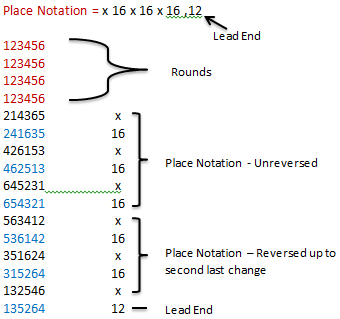
\includegraphics[width=90mm]{Guide.png}}
\subfigure[Figure B]{\label{fig:Complete Method}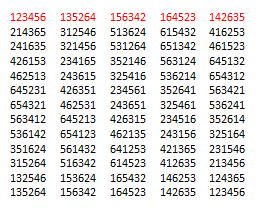
\includegraphics[]{CompleteMethod.png}}
\caption{Example Method}
\end{figure}

%%%%%%%%%%%%%%%%%%%%%%
% http://www.billp.org/bells/crm.php
% http://www.methods.org.uk/other/paca7906.htm
% http://www.jaharrison.me.uk/Ringing/Simulators/
%
%
%
%
%
%
%
%%%%%%%%%%%%%%%%%%%%%%%%%%
\section{Existing Technology}
There are a number of available bell ringing simulators that have graced the bell ringing world in recent years but also 

\subsubsection{John Carter}


\subsubsection{Peter Cummins}
In the 1970's, Peter Cummins set about creating 

\section{Outline}
The rest of the project will consist of :

\begin{itemize}
\item Chapter 2 - Design
\item Chapter 3 - Implementation
\item Chapter 4 - Testing
\item Chapter 5 - Evaluation
\item Chapter 6 - Conclusion
\end{itemize}

\chapter{Requirements}
Requirements describe what the system is supposed to do based on the needs of the customer.  Requirements care not for how the problem shall be satisfied but are statements about what needs done in order to satisfy the problem. With the source code and application available for perusal, after a period of using and understanding the application Functional and Non-Functional Requirements were drawn up.

\section{Functional Requirements}
Functional Requirements define exactly what the system needs to do. They are abstract enough so that End-Users can understand them but also specific enough that the developers can design to that specification.

The MoSCoW principles are used to categorize requirements into levels of importance that can be agreed with the stakeholder.  "Must be", "Should be", "Could be" and "Would be" are the levels of importance that can be applied and after taking time constraints into consideration the main stakeholder agreed on the following requirements.  

%%%%%%%%%%%%%%
%  MUST HAVE %
%%%%%%%%%%%%%%
\subsection{Must Have}
The following are considered to be "Must have" requirements these should be implemented at all costs. They are central to the application and it will be rendered useless without the following.

\begin{tabular}{| l |  p{4cm} | p{11cm} | }
\hline
\textbf{ID} & \textbf{Requirement} & \textbf{Description} \\
\hline
\hline
FR-1 & Stage Selection & The User must be able to select the Stage they wish the method to be \\
\hline
FR-2 & Composition Selection & The User must be able to select what type of Composition the method will follow \\
\hline
FR-3 & Bell Type Selection & The User must be allowed to choose what type of bell they will ring the method on \\
\hline
FR-4 & Peal Time Selection & The User must be able to select the Peal Time for a particular method \\
\hline
FR-5 & Method Ringing & The User must be able to ring a method of their choice\\
\hline
FR-6 & Bell Selection & The User must be able to select the bell or bells they wish to ring \\
\hline
FR-7 & Bell ringing & The User must be able to ring the bell(s) they have selected to ring \\
\hline
FR-8 & Display Changes & The system must display the changes made and guide the user on the path of their bell through the method whilst ringing\\
\hline
\end{tabular}



\begin{tabular}{| l |  p{4cm} | p{11cm} | }
\hline
\textbf{ID} & \textbf{Requirement} & \textbf{Description} \\
\hline
\hline
FR-9 & Method Standing & The system must allow the user to bring a method to a stand at any point while ringing the method\\
\hline
FR-10 & Start Method Changes & The system must allow the user to start the method at any point whilst ringing rounds\\
\hline
FR-11 & Show All Changes & The User must be able to see the complete methods changes for any given method \\
\hline

\hline
\end{tabular}

%%%%%%%%%%%%%%%
% SHOULD HAVE %
%%%%%%%%%%%%%%%

\subsection{Should Have}

The following are considered to be "Should have" requirements and carry a high priority.  These requirements should be included in the final release of the software otherwise it will not be deemed fit for purpose.  

\begin{tabular}{| l |  p{4cm} | p{11cm} | }
\hline
\textbf{ID} & \textbf{Requirement} & \textbf{Description} \\
\hline
\hline

FR-12 & Method Shortlist Selection & The User should be able to choose a method from a user-defined shortlist \\
\hline
FR-13 & Method Shortlist Addition  & The User should be able to add methods to a user-defined shortlist \\
\hline
FR-14 & Method Shortlist Removal  & The User should be able to remove methods from a user-defined shortlist\\
\hline
FR-15 & Stop At Rounds & The User should be able to choose whether the method will stop when it comes back to rounds \\
\hline
FR-16 &  Handstroke Gap Toggling & The User should be able to choose whether the method will include the handstroke gap \\
\hline
FR-17 &  Wait For Me Toggling & The User should be able to choose whether the method will wait for user if they haven't played their bell \\
\hline
FR-18 & Score Blows & The User should be able to choose whether their presses will be scored or not \\
\hline
FR-19 & Score Summary Toggling & The User should be able to choose whether they will receive an average score at the end \\
\hline
FR-20 & Orientation Locking & The User should be able to lock the orientation of the whole app \\
\hline
FR-21 & Back To Rounds & The system should allow the User to go back to ringing rounds at any point during the method\\
\hline
FR-22 & Display Bobs \& Singles & The User should be able to see what path each bell will take during a Bob or Single\\
\hline
FR-23 & Bob \& Single Notification & The system should make the user aware whether it will bob, single or stay as the plain course\\
\hline
FR-24 & Method Pausing \& Resuming & The system should allow the user to pause a method as well as resume ringing that method\\
\hline
\end{tabular}

%%%%%%%%%%%%%%
% COULD HAVE %
%%%%%%%%%%%%%%
\subsection{Could Have}

The following are considered to be "Could have" requirements and carry a lower priority.  They are not requirements of utmost importance but could be implemented if the time frame allows for it.

\begin{tabular}{| l | p{4cm} | p{11cm} | }
\hline
\textbf{ID} & \textbf{Requirement} & \textbf{Description} \\
\hline
\hline
FR-25 & Touch Of Spliced & The system should allow the User to select multiple methods and splice them together as a Composition option\\
\hline
FR-26 & Method Editing & the User should be able to edit the place notation of a method\\
\hline
FR-27 & Bob \& Single Editing & The User should be able to edit the pattern a bob or single will take for any method\\
\hline
FR-28 & Display Alternative Method Path & The User should be able to see an alternative view for seeing the paths of selected bells through the whole method\\
\hline
\end{tabular}

%%%%%%%%%%%%%%
% WOULD HAVE %
%%%%%%%%%%%%%%

\subsection{Would Have}

The following are considered "Would have" requirements and would be nice to have in the final release but look unlikely from outset. They are requirements that should be considered given any future release of the product.

\begin{tabular}{| l | p{4cm} | p{11cm} | }
\hline
\textbf{ID} & \textbf{Requirement} & \textbf{Description} \\
\hline
\hline
FR-29 & Method Updating & The system should update/add/delete methods based on the official list of methods\\
\hline
\end{tabular}

\section{Non-Functional Requirements}

Non-Functional requirements relate more to system properties than what the system should actually do.  They often rely on the needs of the user that are externally related to the system.  They are usually more focussed on things like reliability, performance and depending on the system being designed, if not adhered to can make the system unfit for purpose.\footnote{http://www.sqa.org.uk/e-learning/SDM03CD/page\_02.htm}  

\begin{tabular}{| l | p{3.3cm} | p{11.6cm} | }
\hline
\textbf{ID} & \textbf{Requirement} & \textbf{Description} \\
\hline
\hline
NFR-1 & Portability & Should run on all Android devices supporting API version 14 or above\\
\hline
NFR-2 & Storage & The application should not take up any more than 15Mb in storage costs\\
\hline
NFR-3 & New OS Support & The application should run on the newest version of the Operating system, currently Kit Kat\\
\hline
NFR-6 & Memory Light & The application should avoid using system memory where possible\\
\hline
NFR-7 & Device Size & Should support the various widths and screen densities of devices, including tablets\\
\hline
NFR-8 & Orientation Support & Should support both portrait and landscape \\
\hline
\end{tabular}

\chapter{Design}

This chapter discusses some of the fundamentals about the Android OS, explaining the Architecture that defines an application and some of the key components behind it.  It also discusses some design decisions that were made prior to implementation that have an impact on the project throughout.

\section{Model-View-Controller}
The Android architecture is based on the \textit{Model-View-Controller }(MVC) framework which breaks up the application into more manageable components.  MVC states that every object must either be a Model object, a Controller object or a View object and the interaction that takes using Model-View-Controller can be seen in Figure \ref{mvc}.

\begin{figure}
\centering
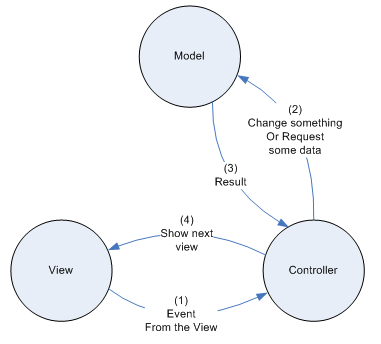
\includegraphics[height=7cm]{mvc.png}
\caption{Interaction between components in the MVC framework. Image taken from: http://www.jadbox.com/2009/03/further-reading-on-design-patterns/}
\label{mvc}
\end{figure}

\subsection{Model}
Model classes attempt to model things that the application is concerned with, so the Model will hold all of the application data or sometimes known as business logic.  Model objects have no knowledge of the User Interface, their only purpose is to store and manage the data. In Android, the Model objects tend to be the custom Java classes that the developer will create.

\subsection{View}
Views objects understand how to present themselves to the user on the screen.  They are a particular representation of the underlying data and this data can be viewed in many different ways. Views also understand how to respond to user input, such as button clicks and swipes.  In Android, there are a whole host of available Views such as Buttons, Linear/Relative Layouts, TextViews. The developer can also create Views to mould the interface as he sees fit.

\subsection{Controller}
Controller objects are the glue that holds the View and the Model together.  They contain the "application logic" and are responsible for the flow of data between the View and the Model layer and vice versa. They are also responsible for managing events that have been triggered by objects in the View layer. In Android, the main controller objects are Activities and Fragments.

\subsection{Interaction}
The interaction between objects in MVC can be seen in Figure \ref{mvc}, the Controller sits between the View and the Model acting as a mediator between the two.  The result being that the Controller controls all data flow between the two and neither will talk directly to each other.  When a user interacts with the View, the View must first send a message to the Controller.  Based on that message, the Controller can then update the data stored in the Model layer if need be and also access any data that it needs from the Model.  The Controller can then update the View based on the new data and those changes will now be visible to the User.  

\subsection{Benefits of MVC}
There are a number of benefits when using a framework like MVC and a few are listed here.

Applications often require thousands of lines of code, and hence using classes and methods helps breaks the problem up into smaller components. As the number of classes gets larger, the more troublesome it can become to make changes to existing code. By breaking classes up into the Layers of MVC, it helps to deconstruct the problem into even more manageable steps and it is easier to describe how aspects of the system will interact.

MVC also makes classes much easier to use and it restricts the scope of its classes; a class that has full access to the application is more problematic than one whose access is limited. 

The use of MVC also makes for much more extendible and adaptable code because of the separation of logic.  View classes need not know anything about the underlying Model layer and hence, should the Model layer choose to represent something differently, it has no effect on the View. One Layer can be changed without needing to change anything from the others as long as it follows the same API. When attempting to support multiple platforms, the only layer needing changed is the layer that interacts with the operating system and in the case of Android, this is all taken care of by Android itself.

\section{Android Architecture}
Now that we have seen a high-level view of Model-View-Controller, we will now delve deeper to see how specific Android components fit into the framework. This section will describe the architecture of an Android application making clear some of the vital components that must be present for an application to function.  

%%%%%%%%%%%%%%
% PROOF READ %
%%%%%%%%%%%%%%

\subsection{Activities}
Activities are application components that provide a screen to the user allowing them to interact with it.  A window is given to an activity in order to create its UI.  Applications will consist of a number of activities that are able to interact with one another.  Activities can start other activities and this forms the flowing from one screen to another.  

Activities have a lifecycle and this is how the activity is notified to changes. This allows activities to let go of resources when not in use and to regain them when pulled back.  The lifecycle can be seen below.


\begin{figure}
\centering
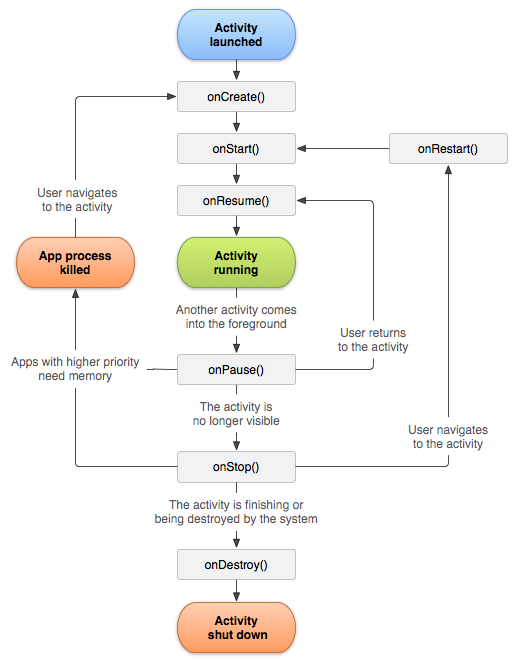
\includegraphics[height=8cm]{activity_lifecycle.png}
\caption{The Activity Lifecycle.  Image taken from:  http://developer.android.com/reference/android/app/Activity.html}
\label{Activity Lifecycle}
\end{figure}

Activities are also responsible for inflating Layouts which give the data a specific structure.

Activities are the main Controller classes in an Android application using an MVC framework, the Controller will interact with both the Views and Model layers. Therefore Activities will interact with the Java classes containing the main application data as well as interacting with Layouts.

\subsection{Layouts}
Layouts describe the visual structure that UI elements will take when they are presented to the user on-screen and can be thought of as Views in a MVC framework.  These are mainly defined in XML files and the components that are defined can be mapped directly to  View classes or subclasses which can be manipulated in the code. These layouts are instantiated at run-time and an activity must specify that layout to inflate.  

Because of this mapping to the View class and subclasses, a developer need not specify their layout in the XML file but rather generate it all within the Activity.  In some cases this is necessary but it is recommended that where possible, layouts should be defined within the XML files.  Because of the flexibility given by the Android framework, both approaches can be used together, specifying some aspects of the layout in the XML and generate the rest programmatically.

Due to the separation of XML from code, devices with different screen sizes and languages can have their own XML file. Recompiling is unnecessary and this eases the burden on the developer.  

\subsection{Fragments}
Fragments in some senses are not central to an Android applications, applications can be created without them unlike Layouts and Activities which an application can not function without. However, in order to ensure a flexible application that can optimize for different devices and allow the use of advanced features then Fragments are a must. 

Fragments are similar to Activities and can be thought of as a subclass of an Activity. It is the other main controller class in the MVC framework that allows the separation of components into reusable pieces.  These fragments are contained within an Activity, and it is said that an Activity will host a Fragment or multiple Fragments.  They look similar to activities but they have a different lifecycle to an Activity.

\begin{figure}
\centering
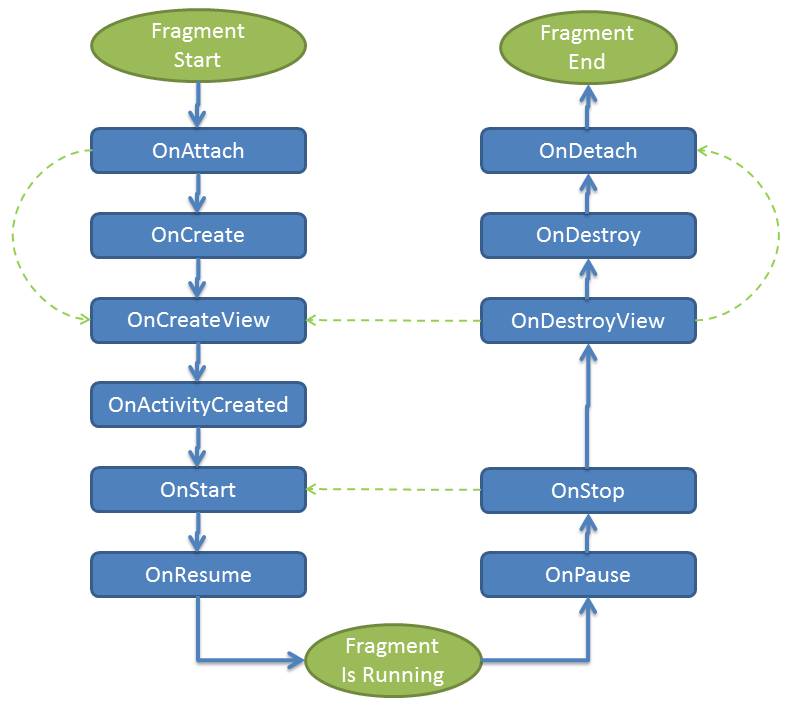
\includegraphics[height=6cm,width=7cm]{fragment_lifecycle.png}
\caption{Fragment Lifecycle :http://docs.xamarin.com/guides/android/platform\_features/fragments/part\_1\_-\_creating\_a\_fragment/}
\label{Fragment Lifecycle}
\end{figure}

With the growing popularity of Tablets, the importance of Fragments was truly realised.  Fragments allow for different experiences on Tablets and Phones. With Activities alone, only one screen can be displayed on phones and tablets however, an activity can host multiple Fragments and hence for a Tablet, Fragments can displayed side by side allowing Android to utilise the extra space offered by devices with greater screen sizes. These Fragments can be simultaneously updated in real-time, touching an option in one fragment can update the contents of the other. This functionality also comes at no cost, there is no need for extra implementation and this one reason to consider them as a central component of an application. 

Even in the case that an application is only being designed for Phones using Fragments would be advised.  Should the day come when you wish that application to made availible for Tablet, it will come at very little cost. 

There are also a number of advanced features in Android that are only available when using Fragments. ViewPagers are helpful UI components that allow the user to swipe between options and using Fragments this becomes very simple.

The final reason that Fragments can be considered as a central component to Android applications is down to the way they deal with rotation. Retained fragments are not destroyed when the device rotates.  Android considers a rotation a configuration change and therefore sets about reloading Activities and Fragments.  This means that they are completely destroyed and recreated but Retained Fragments are not destroyed across rotation.  The View component is recreated but the instance variables are all retained allowing the Fragment to pick up where it left off.  

\subsection{Others}
\subsubsection{Threads}
In an Android applications one main thread will run infinitely that deals with all the processing to do with the User Interface and events triggered by the User Interface.  If a task running on the main thread takes a while to complete then the User Interface is frozen until that task is finished and can sometimes result in an error, namely, an Application Not Responding error which will consult the user asking if they wish to close the application as it is not responding. 

To free the main thread from processor intensive or slow tasks, a background task can take the burden. In Android this background task is known as an AsyncTask. AsyncTasks are extremely helpful for tasks that require connections to servers or for file handling but can run into problems when sharing resources.  To solve some of the concurrency issues, Android will not allow a background task to directly make any changes to the UI, any changes that need made must be given to the User Interface who will service these requests when it sees fit.

\subsubsection{Intents}
In order to communicate with another component Intents can be used as objects for messaging.  Their main use is for starting another Activity and it allows the transfer of data from one to the other. It has other functionality which allows the starting of Services or the delivery of a broadcast.

\subsubsection{Android Manifest}
The Android Manifest is an XML file stored at the root directory and contains a lot of important information and it essential glues the application together. It contains information that the system must be made aware of in order to run the application successfully such as: Classes that implement components, Activities and parent Activities, application permissions, Android API levels and libraries that the application uses. 

\section{Design Decisions}
When an application exists on one platform, the task of creating that application to a different platform becomes be very tricky and can often require meticulous planning and designing to ensure there similarities. It is very difficult to generate the exact same UI layout and in some places functionality and therefore a number of design decision needed to be made, early on, and throughout the project.  The source code of MOBEL was available and the orginial project specification was to port the application to Android.  

\subsection{Porting MOBEL} 
The source code of MOBEL was available from the outset and originally the project was to port MOBEL to Android.  Porting MOBEL to Android would require that the high level structures used in the iOS version be maintained and simply "translated" into Java code.  Porting would also require the UI to look identical where possible given the different platforms. The biggest advantage of doing so would mean that the main application logic need not be re-designed therefore easing the burden during implementation. 

The decision however was made that the application would not be ported to Android.  The application would be re-designed to fulfil the requirements specification but no high-level structure from MOBEL needed to be implemented.  This would mean a complete re-design and coding of application logic and the following subsections outline the rationale behind it. 

\subsubsection{Development Experience}
With Android being a completely new concept, understanding how applications were created and how key components fitted together took  a lot of time and effort. Experience in Java however was a catalyst in picking up Android and meant that some more advanced concepts were feasible early in development.  However, with no experience using ObjectiveC, trying to interpret the source code was particularly strenous. As well as the lack of knowledge using ObjectiveC, there was also the lack of expertise in iOS application development. Therefore, in terms of develpoment experience alone, it was enough to veto the decision to port the application.

\subsubsection{Translation Anomalies}
There are a number of slightly more specific and low-level reasons that porting is difficult from Android to iOS.

Firstly, User Interface Layouts. Android's RelativeLayout and LinearLayout make for a flexible UI given the multutide of screen sizes Android has to cater for.  Behind this is an XML file denoting the structure of any given UI component.  Achieving this flexibility for iOS however is not so simple.  iOS uses an XIB file which has a similar structure but is much more rigid in what the layout can be  \footnote{http://nfarina.com/post/8239634061/ios-to-android}.  This can require a programmatic approach to simple aspects of the UI, such as smooth scrolling which need not be done programmatically on Android.  These subtle differences make interpretting the XIB files troublesome and is another reason behind the choice to veto porting.    

Secondly, Action Bars and Hard/Soft Buttons. Given the simplicity of an Apple device, having the single "Home" button with one or two others for screen locking and volume adjustment, a developer must ensure that all options are availible via buttons on the UI.  Android devices on the other hand have the addtional "Back" and "Options" buttons, either hard or soft.  This allows developers to remove certain logic from the application and attach them to these buttons, often making for a simpler and more effective UI.  Although these differences may not be significant enough to choose to veto porting, compounded with the other reasons it was certainly a factor.

Finally, Activities(Android) and ViewControllers(iOS). They are both focussed things that the user can do and serve as the main logic in an application. The two big differences between them are the methods attached to them both and the level of control of the lifecycle.  Android offers a different set of methods in order to control and create its Activities to that of iOS as well as offering much more control in terms of its lifecycle. Again, this is no reason to veto porting on its own but still served to make the decision easier.

\subsection{Modifications}

\subsubsection{Home Screen}
The Home Screen of an application is where the User will find themselves when they load up the application. MOBEL chose to have the home screen set as the screen where the users would ring the bells.  This meant that if the user wished to change any of the settings they would have to hit the "i" button in the top left hand side of the screen. The decision therefore to change the Home Screen was one that was made early on in the interests of usability.  

The decision was made to use the Settings page as the Home Screen.  This allows the user to select all the settings they wish before actually going to ring that method.  It is also a reminder to the user as to what settings were used earlier as the "ring Method" Screen contains little information regarding the users choices. In some situations, the Home Screen will not be the first to open thanks to the Android OS.  If a user is to hit the "Home" button then the Activity is still stored in memory.  Should the user choose to come back and use the application again it will load the application from memory and will start where the user left off.  If the user closes the application or it has been sitting idle in memory for long enough, the OS will free up the space for another application and therefore MOBEL must be booted from disk.  This will ensure that MOBEL will start at the Home Screen once again.

\subsubsection{Ring Button}

\subsection{API Version}
The API version of an Android application is incredibly important as it governs what devices are able to install that application.  If a device  attempts to install an application with whose minimum API level is higher than that of the devices, it will fail.  Due to the ever changing nature of Android, this can render older devices redundant very quickly.

One of the central UI features of MOBEL is the switch, a boolean component allowing the user to choose between one of two options.  This was a standard iOS component, availible in much older versions of iOS.  Android on the other hand didn't integrate the Switch into their SDK until API version 14 was released.\footnote{http://developer.android.com/reference/android/widget/Switch.html} 

There was now a trade-off between portability and likeness to MOBEL, cost between satisfying the needs of older devices or a cleaner UI with more obvious similarities to its sister application.  

Roughly 21\% of all Android devices still run on a lower API level than version 14 with the majority running Gingerbread. The decision was to go with the UI look and feel rather than that of the applications backwards compatibility.  After a discussion with a stakeholder in the system, the client felt that the Switch was a much needed aspect of the application.

\subsection{MediaPlayer vs SoundPool}
One of the key aspects of the whole application is the ability to ring sound clips. The audio recordings of the bells are short, most being under 1 second of recorded audio.  The application requires that the sounds be played in real-time, very quickly one after the other.  This can be a strain on the device itself as MOBEL sometimes encountered irregularities during playing.

\subsubsection{MediaPlayer} The MediaPlayer class provides a framweork for developers to integrate audio and video playback into the desired application.  It can be used to play media on the local file system and also in the applications stored resources.  When playing audio it streams it from media rather than from memory and hence there can be a noticeable lag between set-up time and playtime.    

\subsubsection{SoundPool} The SoundPool class makes use of some of MediaPlayer's functionality, allowing the audio to be decoded into a raw 16-bit PCM stream.  The advantage being that the CPU doesn't suffer  a higher load or decompressing latency while the audio is wishing to be played. SoundPool also offers a "pool" of sounds that can be rendered at once.  A SoundPool object should be created before the main process has started, therefore the more CPU intensive tasks are done early and the sounds are prepared for the when the system requires.  SoundPool has been optimized for short sounds that can be played on top of each other with there being a 16Mb limit on the SoundPool.

\subsubsection{Conclusion}
Testing showed that due to the clunky, processor intensive nature of the MediaPlayer, it became unsuitable to use.  There were often irregularities during playback and as the application progressed further through playing a method these became more obvious. When audio was playing at a high tempo, there came a point where MediaPlayer could no longer cope and the audio stopped altogether. It became apparrent that MediaPlayer was unsuitable and further testing begun when using SoundPool.  Because of its short sound optimization, decompressing the audio and storing the raw audio in memory, it meant that the response and play time was incredibly fast.  Sounds played fluently over each other and in a regular pattern. Testing showed SoundPool to cope even when the tempo was set higher than the application would actually allow. 


http://developer.android.com/reference/android/media/MediaPlayer.html
http://developer.android.com/reference/android/media/SoundPool.html
http://www.stealthcopter.com/blog/2010/08/android-soundpool-vs-mediaplayer-focus-on-soundboards-and-memory-problems/


\section{Design Patterns}
A design pattern is a recognised, formalised, reusable solution to a recurring problem when designing software. Using design patterns in Software design makes for stronger code but in general helps develop a more robust, clean and usable application.  Looking at the task ahead in implemented the system, based on the iOS application the following design patterns seem feasible to use and should be adopted where possible.

\subsection{Singleton}
A Singleton object is a wrapper around another object that ensures it can only be instantiated once. Rather than having a public constructor that can be used to create the object, it has a public static method (often \textit{get()} or \textit{getInstance()}) which will return the instance of the object that you want made a Singleton.  It does this by removing access to a public constructor and instead controls its use using a private constructor.  The get() method will check if the object it is encapsulating has already been instantiated. If the object has not been instantiated it will use its private constructor to create the object and return that to the user.  If it has been created already, it will just return that object. Because of the tight controls on the constructor, it is easy to see how only one can be created. 

\subsubsection{Benefits}
The main reason Singletons are popular amongst Android developers is because of their longevity of life and accessibility. In an application where Activities and Fragments are constantly being created and destroyed, there often needs to be some base data that is available to all the Activities. Using Intents, data can be passed from one Activity to the other but this is often messy and for large data can have some performance issues.  It also couples the data to those specific activities and should a developer wish to edit the application later in time it can be problematic to make additions.  The Singleton object on the other hand will remain in memory until the application is closed. This provides the consistency needed to share data access across all Activities and Fragments.  

Looking at MOBEL, it can be seen that methods need to be accessed nearly everywhere in the application, and even at this early stage, a singleton object looks as though it will prove useful to service all the different screens. 

\subsection{Adapter (Decorator) Pattern}
The Adapter pattern, sometimes known as the Decorator pattern, is a wrapper class that allows two classes to interface together that would not be able to otherwise. When one class tries to communicate with the other, it stands as a mediator between the two, translating that of the request into something the Adaptee can understand.  It becomes very useful for transforming data into the appropriate form for the Adaptee.

\begin{figure}
\centering
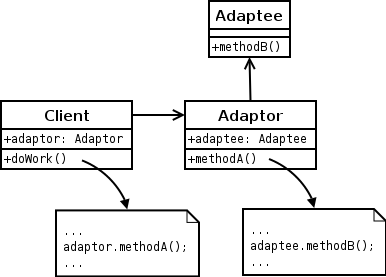
\includegraphics[height=5cm]{ObjectAdapter.png}
\caption{Adapter Pattern.  Image taken from: http://en.wikipedia.org/wiki/Adapter\_pattern}
\label{Adapter}
\end{figure}

\subsubsection{Benefits}
Adapters in Android are useful for binding Views to the data it is going to display.  Adapters are used in Android when working with ListViews, which are the most popular way to display large amounts of data on-screen. The ListView wants a series of Strings so it can display each and the Adapter does all the hard work for the developer. It takes an Array of Strings and maps them all to a different View within the ListView.  If a View is deleted, then it is also removed from the array.

Looking at MOBEL for iOS, there are numerous occasions where a list of data is presented to the user.  Therefore the Adapter pattern should be used by taking advantage of Android's own Adapters and ListViews, rather than attempting to write a custom Adapter unless it is entirely necessary. 

\chapter{Implementation}

\section{Set-up}

This section describes the implementation of foundational concepts that are set-up related.  This refers to the selection of methods, addition of methods, selection of stage, composition, peal time etc as well as the displaying of method changes and bobs/singles.

\subsection{Shortlist}
There are thousands of possible methods that a user can ring and finding these methods would be particularly troublesome if they would have to scroll through a lengthy list of all methods.  MOBEL thankfully breaks this up to make finding these methods much easier.  

Methods are first split by Stage.  The User is required to choose their stage on the Home Screen and hence MOBEL knows only to load in methods of that particular stage.  Methods are then split by type, this again allows for a much better filtering of results and reduces performance overhead.

Even with the introduction of these filters, some method types still contain well over one thousand method and therefore it becomes unfeasible to ask the user to have to wade through a massive list to find their chosen method. MOBEL's answer to this problem was to introduce a user defined shortlist whereby a user can create their own list of methods and choose their method from that list.  
\subsubsection{Benefits}

The introduction of the shortlist allows users to tailor the application to their own personal taste, storing the methods they use or like most and reduce time spent in set-up and maximise time spent ringing. It makes the application much more useable, whereby users are not left disheartened having to scroll through a long list to try get to the entries that lie in the bottom half.

The benefits for the user are evident but there are also noticeable performance benefits for the application.  Some method files are so long that it can take up to 3 seconds for the MOBEL to read them in from file and display them using the listview. This 3 second wait only need happen when the user wishes to add that methods of that specific type to the Shortlist, whereas without the Shortlist is would need happen any time the user wished to ring a method of that type. 

\subsubsection{Implementation}
The way to create this shortlist is essentially to cache the methods in a small file so they can be read in much more quickly than the large file. Every time the user adds a method to the shortlist, the current methods in the shortlist are written to file.  Each time the user wishes to select a method, when the Method Selection Screen is loaded up, the file is read in from backing storage and the methods are displayed on screen. 

A custom view was created for the 


\subsection{ListView}
On most mobile devices, the user will often need to choose an option from an available list.  MOBEL is no exception being an application that is highly customizable with a large number of choices that impacts the user experience. The ListView is used in the selection of additional methods as well as the selection of Composition and Stage.

\subsubsection{Performance}
Non-Functional Requirement 5 stated that the application should preserve battery where possible and Non-Functional Requirement 6 stated that the application should avoid using System Memory where possible. ListView are what can be used to ensure that these non-functional requirements are adhered to.  

Layout inflation is expensive using Android and inflating a complex or large layout can take a considerable amount of time, often due to the devices hardware restrictions. ListViews are what Android recommend to use when displaying a list of options to the user.  It is possible to do without listviews by inflating the Views themselves inside of a ScrollView.  Should the number of Views be large, it may take a number of seconds to inflate them and display them on screen. 

In order to save memory and also processing power Android recycles Views.  Rather than creating a View for every option in the list, it recycles old Views to save on the costly inflation operation and storage space. Android will inflate Views containing the Users current options and also some extra options so that when a User scrolls Android can quickly bring that View in from memory.  The options that are now out of view can then be recylced to contain new content and will be brought into view when the user scrolls even more. Figure \ref{ListView} shows the structure of a ListView.


\begin{figure}
\centering
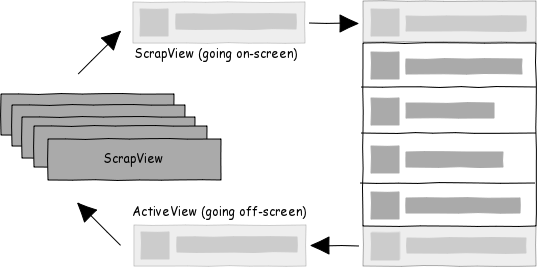
\includegraphics[height=4cm,width=7cm]{listview1.png}
\vspace{0mm}
\caption{ListView}
\label{ListView}
\end{figure}

\begin{figure}
\centering
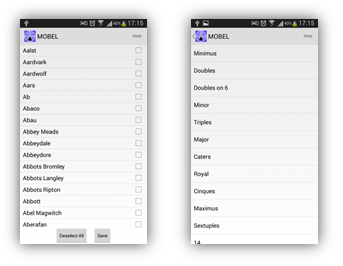
\includegraphics[height=5cm]{ListViews.png}
\vspace{0mm}
\caption{Examples of ListViews in MOBEL for Android}
\label{listviewAndroid}
\end{figure}

The ListView is used many times in MOBEL but there is one clear application of its use that was a great benefit to the project.  A User is able to add a method to his personalised shortlist from a list of all Methods of a certain type.  Some Method types contain a large number of methods to choose from (e.g Surprise Major) with hundreds of possible choices.  Testing showed that without the use of a ListView it could take nearly 40 seconds to inflate and display all the methods in their own view.  The ListView in this case ensured that the main thread did not hang and that the application was not memory intensive.
\subsubsection{Scalability}
Scalability is another aspect of the ListView that can be exploited during future development. If at any point the application allows updating and additional methods to be added then the developer can be sure that applicationm performance will not be hindered when using ListViews.  This makes the application extendible and ensures that Non-Functional Requirement 4 is adhered to.



\subsection{Drawing Lines}
\subsubsection{Requirement}
Functional Requirement 11 states that the user should be able to see all the method changes for any given method. The User has the option to see this screen when they are choosing a method from their custom shortlist or also after they have chosen it, by selecting the "Show" button on the ring method screen.

To display the method changes, a TextView would be required to display the numerical changes that each bell takes.  In MOBEL however, a different coloured lines follow the path of the treble and bell 2 through the method.  MOBEL also shows an alternative view should the user press the screen where just the coloured lines display the pattern of changes through the method with the numerical changes not visible. Both views can be seen in Figure \ref{Lines}, the alternative view being that on the right hand side.

\begin{figure}
\centering
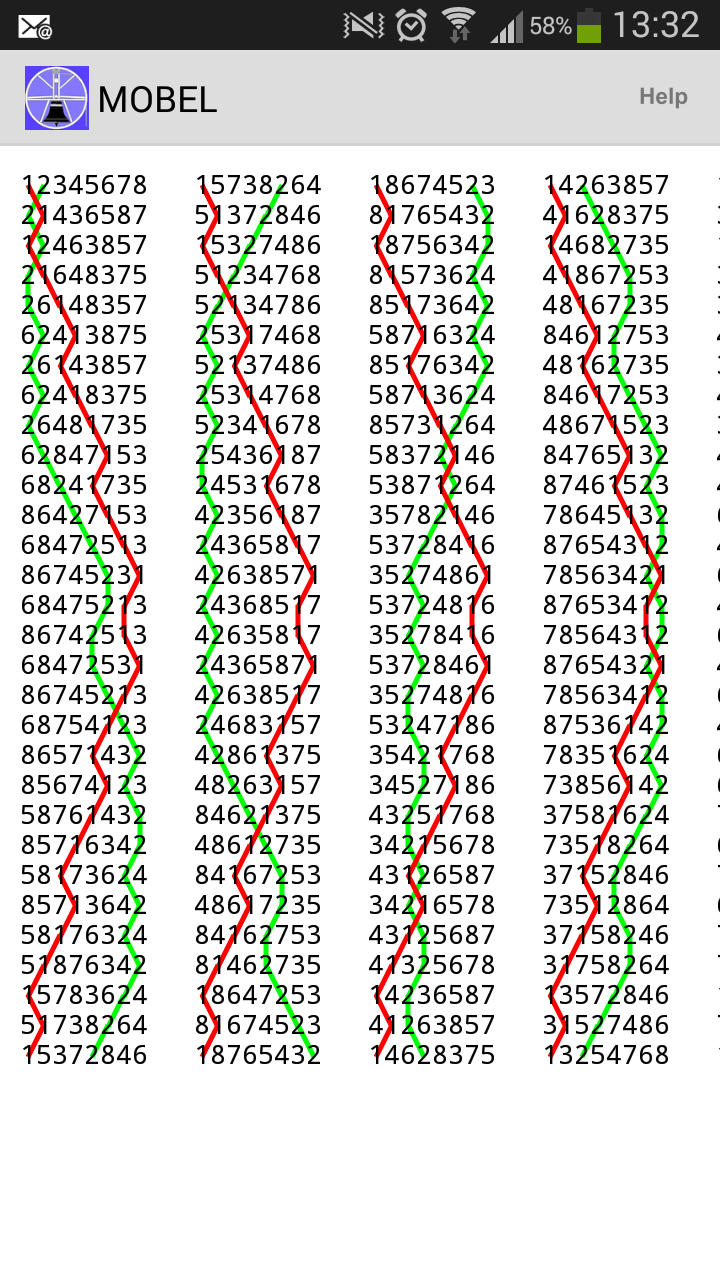
\includegraphics[height=4cm,width=3cm]{lines.png}
\hspace{1cm}
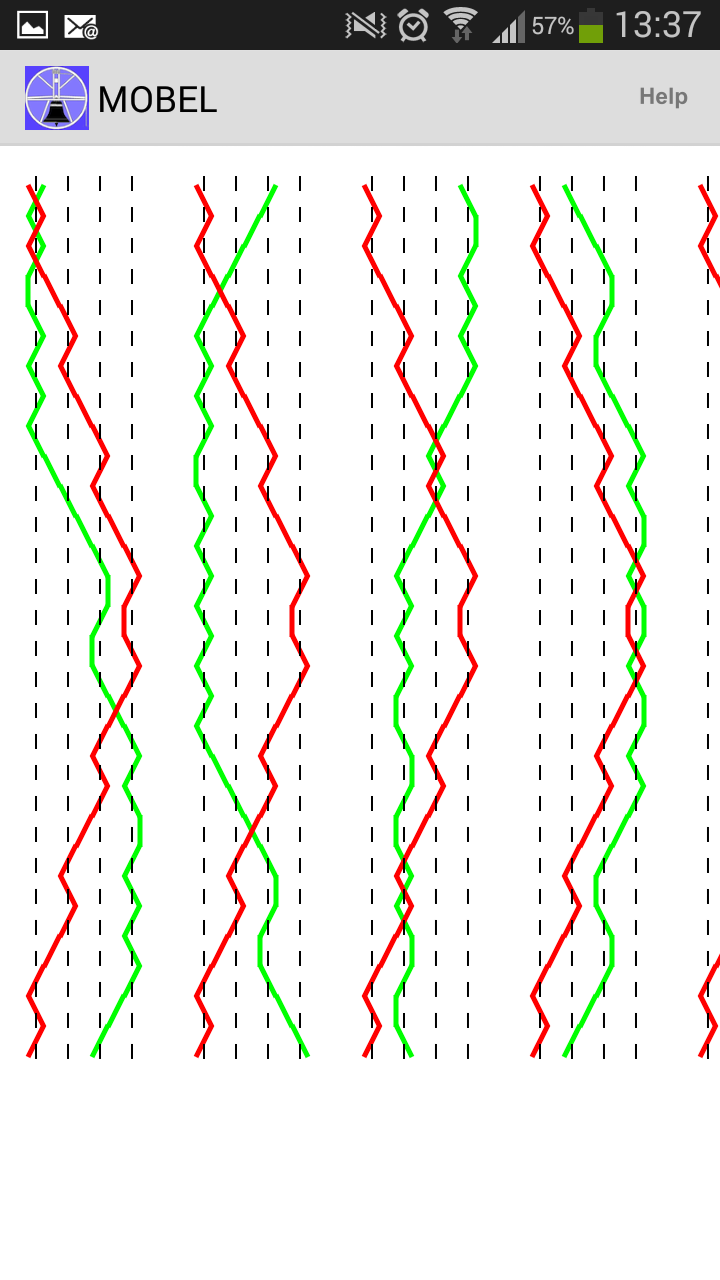
\includegraphics[height=4cm,width=3cm]{lines2.png}
\caption{Lines}
\label{Lines}
\end{figure}

\subsubsection{Implementation}
As was previously mentioned, the TextView class is able to display the numerical changes but not the coloured lines.  However, by extending the TextView class it would allow for the required functionality.  Contained within the TextView class is an \textit{onDraw(Canvas canvas)} method. The Canvas object here is what it uses as a layer on top of the background and is fully customizable.  Canvas contains methods like drawLine() which allows you to draw a line from one coordinate to the other.

\subsubsection{Algorithm}
The algorithm to draw the lines is simple and assumes that all text has mono-spacing applied.  Calculate the position of the first character , x and y.  Using the text, remove the first line ("n" as the delimiter) and loop until there are no lines left. Inside the loop, using the removed line of text find the index of bell 1 and bell 2.  Using the indexes of the previous line, use the drawLine() method and coordinates based on the position of the first character (x = pos\_X\_first-char * index, y = pos\_Y\_first-character * times\_looped) to draw the line. This will successfully draw the lines through the required values. 

\section{ringing Along}
This section describes the implementation of foundational concepts in relation to the user playing the method.  This refers to functionality related to the screen where the bell ringing takes place.  

\subsection{Rotating Images}
\subsubsection{Need For Rotation}
There are two main reasons that the rotation of the bell images on the screen are necessary.  The first is to fulfil Functional Requirement FR-6 which states that the user should be able to select the bell(s) they wish to ring. In MOBEL the users choice of bells to ring will always sit as the bottom two bells in the ring of bells.  This requires the bells to rotate round the circle to preserve the correct order.

The second reason this is done is to make it easier for the user to find the two bells that are being ringed.  Should the bells just assume their starting position, they maybe be in a more awkward place to see.  Having the bells sitting near the bottom of the screen ensures that the user can see their own bells while still watching the changes as the system displays the current position in the method box situated below.



\subsubsection{Implementation}

\begin{figure}
\centering
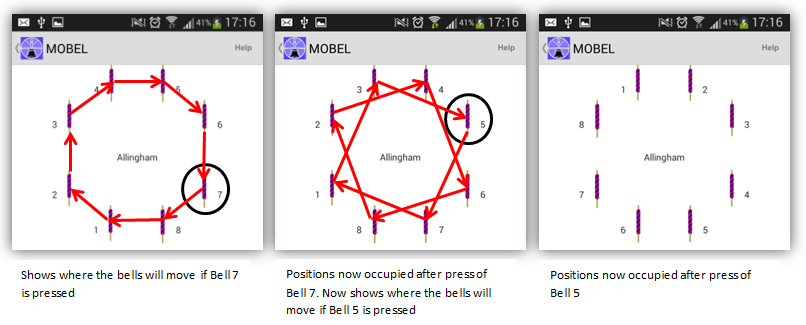
\includegraphics[width=15cm]{Rotation.png}
\caption{What happens during rotation}
\label{Rotation}
\end{figure}
\subsubsection{Algorithm}


\subsection{Sounds}
The actual bell sounds being ringed is the most foundational part to the application, without the sounds the application is rendered pretty useless. As was aformentioned the decision to use SoundPool was made and development began using SoundPool to ring the associated sounds.
\subsubsection{Sound Scheduling}
The first piece of information required to schedule the sounds at the correct time was knowing the Peal Time. Knowing the Peal Time and Stage would allow the calculation to take place which would determine how long a bell had to wait before being played fater the prior bell.  

The formula is as follows: 
\begin{itemize}
\item Peal time = PT
\item Interval between bells = I
\item Number of bells = B
\item Handstroke Gap (On/Off = 1/0) = HG
\end{itemize}

\begin{equation}
I = \frac{PT}{2500\times(2B + HG)}
\end{equation}

Now that the interval can be determined, the time at which a bell needs to sound can be triggered. 

The second thing needed was a way of actually ringing the sounds in a regular fashion.  As was aforementioned, it would be unsuitable to do all of this on the main thread as the user would lose the ability to interact with the UI as long as the sounds were running.  Therefore, a separate AsyncTask was set up to run in the background that would use Handlers to interact with the User Interface.  This task would run as long as the user was playing the bells and upon completion would be destroyed.  Handlers were also used in order for the AsyncTask to interact with the UI in a legal manner.

The final thing then, scheduling.  There are various methods of scheduling the sounds to play inside the background thread each pertaining to their own advantages and disadvantages.  The  chosen scheduling method worked in the following manner. 

\begin{enumerate}
\item Retrieve next bell number
\item Update UI using Handler
\item Play Bell Number
\item Thread wait for I milliseconds (interval between bells)
\item Check for changes in user choices (e.g User pressing Rounds)
\item Loop
\end{enumerate}

The thread in this case waits for the Interval length after playing the bell noise.  This would not be as accurate as setting a time at which the bell must play based on the interval but there is reason behind this methodology.  There are quite a lot of tasks that the AsyncTask must perform between the ringing of bells, most of them are simple however and will be executed in a number of microseconds.  Although there will be a difference in accuracy, it will be kept to a minimum and in rare cases may be more than 1 millisecond.

The main advantages scheduling using this method are firstly to do with background processing of other tasks.  When other actions, like text messages or background updating happen, what can happen is the application

\subsubsection{User Interaction}

\section{Playing}
Allowing the user to play along is another primary aim of the application.  The User must be able to interact with the UI by tapping on the screen to play their respective bell.  The user must also be able to play along with two bells if they have chosen to play using Handbells.

\subsection{Implementation}
When the user starts the bells, they will play on their own until  the user begins to tap the screen.  This way, should the user just wish to listen to the sequence of changes, they can do so without needing to play.  If they wish to play, they will need to  time their bell presses well otherwise it will sound out of place.  For Handbells, the screen is split in two, one sidefor each bell and in a similar manner they can play along or simply leave it to sound through.  

This is implemented using an onTouch() listener.  The listener will sit waiting for any kind of touch event from the user and on doing so, it will trigger the playing of that sound.  The time is also recorded for scoring purposes.  If the user is playing with 2 bells then the coordinates of the press are taken into consideration, if it is on the left side of the screen then the left bell will play and similarly for the right hand side, if a user presses on the right hand side of the screen then the right bell will play.  Other View components listeners are nullified prior to playing so that the user has full use of the screen to touch anywhere

\subsection{Difficulties}
For a period during development, the sound pattern was irregular, pressing the screen had a noticeable lag before the bell would play and this meant that there was something not working correctly.  The reason for this irregularity was not mathematical error but the wrong listener.  An onClick() listener was currently being used as opposed to an onTouch() listener.  The Android OS would have to wait just a fraction of a second to identify if the users interation was a click rather than a hold, or swipe.  The onTouch listener however fires the second it knows the user touched the screen and once this had been recognised, all irregularities in playing along were removed. 


\section{Home Screen}

\chapter{Testing}
This chapter discusses the various means of testing that took place throughout project. Beginning with the chosen method of testing and followed by the various testing means and results of each. 

\section{Testing Methodology}
Without testing, the developer can never know how well the applications functions, feels, looks or whether it is fit for purpose. Testing can often be overlooked but its presence with in Software Development is essential and there are a number of possible development methodologies that shape the way testing is performed.  The following methodologies often relate to the Software Development process as a whole but what is being discussed here is in particular relation to testing within those methodologies.

\subsection{Waterfall Method}
When following the Waterfall method, testing is left until implementation has completed as can be seen in Figure \ref{Waterfall Method}.  The sequential nature of the Waterfall Method results in bugs and deficiencies being discovered much later in the development process and if they are significant enough it can sometimes require a complete restructuring of the application.  

\begin{figure}
\centering
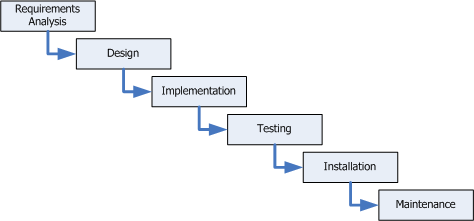
\includegraphics[height=5cm,width=8cm]{waterfall-method.png}
\caption{The Waterfall Method [http://www.projectsmart.co.uk/waterfall-v-agile-how-should-i-approach-my-software-development-project.html]}
\label{Waterfall Method}
\end{figure}

\subsection{Agile Methods}
Agile Methods are more iterative, fluid methods where testing is central to weekly work.  A sprint takes place over a selected period of time in order to release a version of the software with partial implementation. At each sprint, the old version is built on and new features are added, iteratively building up the software until it is complete. Coding and testing flow more dynamically and it ensures bugs are being found throughout the process rather than all being found post-implementation.  At the end of each sprint the software is demonstrated to the clients and the developers can get feedback from the end-users as to how certain aspects of the software could be improved or changed.

\subsection{Chosen Methodology}
There were many factors that affected the choice of methodology but it was clear as to which was best suited. The circumstances of development meant that a meeting was held once a week with a stakeholder, who had good experience using MOBEL for iOS.  This became the platform therefore for an more Agile based approach to development and testing specifically. A sprint would be one week long and would end by having a testing session with the stakeholder. High levels of in-depth feedback could be gathered and adopted into the next sprint and the application would iteratively grow as the weeks  went by. It meant that many small bugs or misunderstands were picked up early in the development process and application development progressed quickly.

\section{Functional Testing}
Other than the demonstrations to the stakeholder, tests needed done so that there was a guide on whether the system was complete or not.  Being a Port of the iOS application, the system would need to function in the same manner as the iOS application to be complete.  Therefore, tests were drawn up to ensure that each of the functional requirements were tested and that once all had been passed, the system would be ready for evaluation.

This testing was performed during the sprint and were performed when the features in question had been added.


\section{Formal User Testing}
With such a wide choice of settings, testing thoroughly can become very difficult.  As the creator of the application, it is easy to overlook parts of the system and to assume it functions correctly when it may fail under certain test conditions.  Therefore, a session of user testing was set-up with some bell-ringers to get a more thorough range of tests.  The bell-ringers themselves, who have a much wider knowledge of bellringing as a whole can therefore understand the purpose and workings of the application as well as providing more in depth feedback.

\subsection{Aims}
It is important to know what the aims for a particular testing session are and what this particular testing was neither a user evaluation nor was it a usability test.  It was a means of Functional Testing, to see whether the system achieved what it set out to do.  Due to the application being a port from iOS, there are constraints set on how the application will look and feel and hence the testing session endured it stayed away from that.

The testing session was also there to try and identify any bugs that remained in the system.  Testing had been done in the past but allowing actual end users to test the software will yield more realistic results.

\subsection{Testing Conditions}
The application was installed on a Samsung Galaxy S3 running Android 4.3.3, and it was also installed on a Samsung Galaxy Tab3 running Android 4.2.2.  The application is to be made available to the public via the Google Play Store upon completion and hence it is important to tests on both Tablet and Mobile devices.

When confronted with a new application, it can be said that most people dive in and learn how to use that application by playing with the application for a period of time. For those who wished to experience MOBEL that way, this was no problem but a User-Guide was made availible to those who wished to use it and can be found at Appendix BLAH.  MOBEL has a lot of subtle options that a user may struggle to find or understand, hence the user-guide was made availible to combat any issues that the bellringers would have in testing.

Finally, a Testing Guidline and Feedback Form was given to each of the users taking part in testing and this can be found at Appendix BLAH.  To ensure that the majority of feedback questions could be answered, a walkthrough was provided that detailed a number of things that users should try to do before using the spplication more freely for themselves.  Users were also made aware of what they were testing, to ensire that there was no confusion and that the results would remain accurate.  
  
\subsection{Reuslts}

The results of testing have been displayed in Figure \ref{Test Results}. Each test relates to a Functional Requirement and the table showing the relationships can be found in Appendix BHA

\begin{figure}
\centering
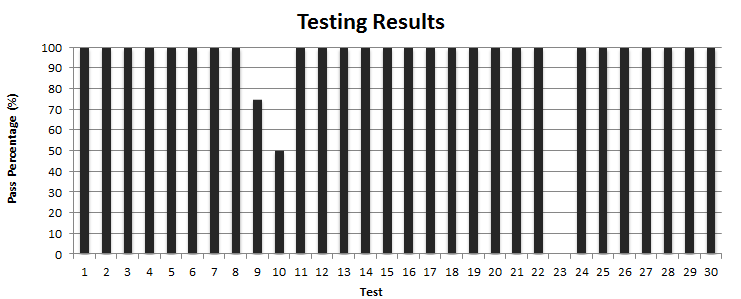
\includegraphics[width=18cm]{testingTable.png}
\caption{Testing Results}
\label{Test Results}
\end{figure}

User-Testing served a useful purpose in discovering three bugs that would have otherwise gone unnoticed. The three tests that failed were: \begin{itemize}
\item Test 9 - "Did MOBEL display the correct changes as you rung through your method"
\item Test 10 - "Did MOBEL allow you to start ringing the method once you pressed 'Go'" and test 
\item Test 23 - "When 'Wait For Me' was selected, did MOBEL successfully wait for you if you never rung your bell"
\end{itemize} 

Testers were encouraged to leave comments should they find the system doing something they felt was incorrect.  Given their comments, the reasons for each bug became apparent and a solution for each was found.

\subsubsection{Bug :Test 9}
Comments stated that when they tapped the screen to ring along, the image of the bell was ringing the incorrect stroke.  Although their is no difference in terms of sound, the difference can be seen visually.

This was a minor issue, but an issue nonetheless. When the User clicks the screen, they will ring their bell and the image of bell will change to the opposite stroke.  When MOBEL starts ringing it always assumes the user will not be playing along so rings its own changes and switches its own images.  When the User chooses to play along and tries to time their first press, if the user strikes slightly late, the system will ring and so will the user and hence the stroke of the bell will be wrong as a double ring was performed.

Ammendments have now ensured that this issue will no longer arise. 
\subsubsection{Bug :Test 10}
Users commented that when 'Go' was clicked, the method should have played an extra set of rounds before going into ringing method changes.

In MOBEL for iOS, when 'Go' is clicked, after the last Handstroke Bell has rung, one more set of rounds will be played before method changes begin.  During this testing session, MOBEL for Android showed that method changes began after the last Handstroke Bell had rung and that it did not play one more set of rounds before starting. 

Changes have been made to the code and thorough testing was done to ensure that the reflected changes now matched the iOS version of the software.

\subsubsection{Bug: Test 23} 
Users commented that when ringing Towerbells with 'Wait For Me' selected, that the system waited for their input but on clicking the screen to continue, the system did not accept their input and that MOBEL continued to wait indefinitely. 

This bug was more subtle than the last and only came to the fore when Towerbells was selected.  When playing Handbells, with 'Wait For Me' selected, the User is required to play with 2 bells and the system waits indefinitely until the user taps the screen.  When playing Towerbells, the system was waiting for a 'second bell' tap on the screen from the user, however, only one bell is played when using Towerbells and no 'second bell' tap was able to be played.  The thread that was therefore waiting for a bell tap that was impossible to play and the thread waited indefinitely. 

Changes were made so that when Towerbells was selected, it no longer was waiting for an input it could not receive.  An additional change was made so that if they user did not play anything for 2 seconds, MOBEL would assume they no longer wished to play along and subsequently would progress through without waiting for input 

\chapter{Evaluation}

\section{Chris Hughes Evaluation}

\chapter{Conclusion}


%%%%%%%%%%%%%%%%
%              %
%  APPENDICES  %
%              %
%%%%%%%%%%%%%%%%
\begin{appendices}

\chapter{Android}

\section{Introduction}

Android is an operating system based on the Linux V2.6 kernel. Androids initial deployment target was mobile-phones, including smart phones and the cheaper flip phones. Androids full range of services and functional support have given way to its use on other platforms and applications.  

Android's use of the its own custom Virtual Machine allows for hardware resource optimization and meticulous memory management.  All Android devices are fully customizable, no application holds precedence over another, which allows even third-party applications to have full access to the devices capabilities.  

The Open Handset Alliance, a group of companies that joined forces in order to build the best mobile phones, are the group that coined Android and went about putting it into development.  The group, led by Google, includes a large number of handset and component manufacturers, mobile operators, software solution and platform providers. In terms of software development, it is one of the largest pieces of software in the Open Source world.

\subsection{Android Beginnings}
The first Android-capable handset on the market was the HTC G1. Shortly before the G1's release, in September 2008,  the first Android SDK was released - 1.0 - and Android applications began surfacing.
To entice development and innovation, Google sponsored two rounds of "Android Developer Challenges" with millions of dollars being offered to the best submissions. Only a few months after the G1's release, the Android Marketplace was released which allowed users to browse and download applications straight to their mobile device.

\subsection{Fragmentation}
Unlike iOS, which is only ever run on devices manufactured by Apple, Android is run on thousands of different devices. This is a blessing in some ways, allowing users a much greater choice of devices, tailored to their own personal preference. In other ways, mainly for developers, this is a pain.  The varying screen sizes (see \ref{ScreenSize}) and hardware configurations making it difficult to predict how an application may look or feel on a different device. Android has ways of dealing with these problems but often comes at the cost of more complex code.

As of March 2013, there have been 19 major releases of Android. The most recent being Android 4.4 Kit Kat (API Level 19).  The most recent version fashioning support for hidden system and status bars, printer support, and lower memory usage. It also has a number of user-level improvements, including a new dialer, a Google-infused home screen, and a whole pile of UI refinements.

\begin{figure}
\centering
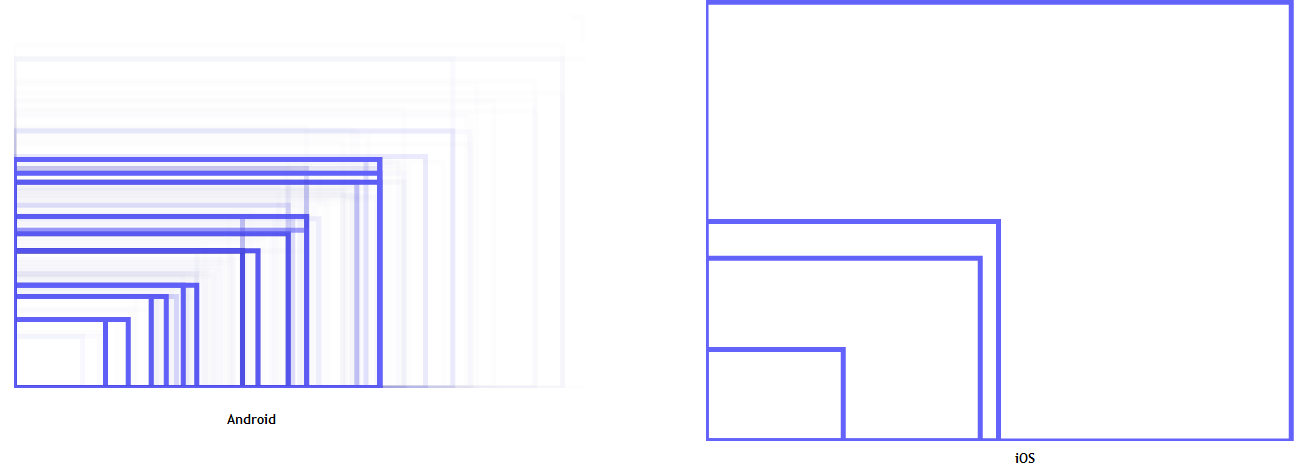
\includegraphics[height=6cm,width=14cm]{sizeComp.png}
\vspace{0mm}
\caption{Screen Size Comparison}
\label{ScreenSize}
\end{figure}
http://www.slideshare.net/softheme/mobile-application-testing-12270081

\section{Development}

\subsection{Language \& Android Architecture}
Android applications are written using the Java programming language which run in a Virtual Machine.  Java itself is an Object-Oriented, Concurrent, Class Based programming language designed to have as few dependencies as possible. Its intention was to be "Write Once - Run Anywhere" which is possible thanks to the Java Virtual Machine (JVM).  Java code, is compiled into Java Bytecode, which the JVM can then use to run the Java program.  It may be surprising to note that Android applications to not run in the JVM, rather, the Dalvik Virtual Machine.  The Dalvik VM is an Open Source technology, and each application runs within an instance of it.  This resides within a Linux Kernel manages process and can be seen in \ref{SoftwareFramework}.

\begin{figure}
\centering
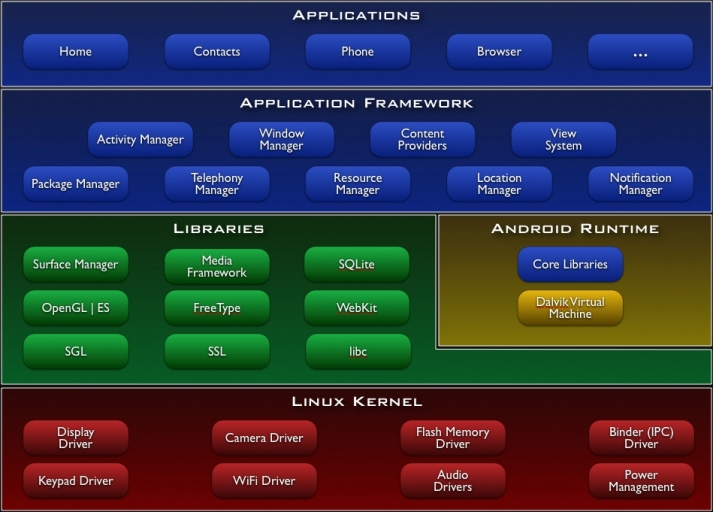
\includegraphics[height=8cm,width=10cm]{android_architecture.jpg}
\vspace{0mm}
\caption{Android Software Framework}
\label{SoftwareFramework}
\end{figure}

\subsection{Development Tools}
Eclipse is an integrated development environment (IDE) containing a base workspace and plug-ins in order to customize the environment. Written primiarily in Java, Eclipse can be used to develop applications and is most popular for developing Java applications. Because Android is programmed using Java , Eclipse is the natural choice of IDE. Development can be done without Eclipse but an excellent understand of the SDK would be necessary in order to do so.  

As mentioned earlier, Android is open source and hence the source code is available for all developers and is called the Android SDK (Software Development Kit). Eclipse has a plugin that makes developing applications easy, the Android Developers Kit (ADT). This allows the installation of the specific SDK, as well as allowing developers to create projects, launch emulators, debug, etc.

Drivers can also be downloaded for Eclipse that allow developers to test Applications on their own mobile device.  Should the developer not have a device to use, Eclipse provides an Emulator to allow testing on various versions of Android on devices with different screen sizes and densities. 

\subsection{Design Patterns}

\subsubsection{Model-View-Controller}

\subsubsection{Observer-Observable}


\chapter{GitHub}

\chapter{Stages}\label{C}
This following list shows for each Stage, how many bells are needed in order to play.

\begin{itemize}
\item Minimus - 4 Bells
\item Doubles - 5 Bells
\item Doubles on 6 - 6 Bells 
\item Minor - 6 Bells
\item Triples - 7 bells
\item Major - 8 Bells
\item Caters - 9 Bells
\item Royal - 10 Bells
\item Cinques - 11 Bells
\item Maximus - 12 Bells
\item Sextuples - 13 Bells
\item 14 - 14 Bells
\item Septuples - 15 Bells
\item 16 - 16 Bells
\end{itemize}

More Stages can be played but MOBEL has been restricted to 16 bells.

\textbf{NOTE:} Most Bell towers across the world will contain an even number of bells.  The exception being that some contain 5.  For this reason, when using MOBEL to play an odd numbered Stage (other than Doubles), it will be played with one extra bell.  This bell will ring last in every row and will not follow any changes that are given.

\chapter{Functional Testing Tests}
\begin{tabular}{| l | p{1.8cm} | p{2.4cm} | p{7.5cm} | p{0.6cm} | p{2.7cm} |}
\hline
\textbf{ID} & \textbf{Related Functional Requirement} & \textbf{Test} & \textbf{Description} & \textbf{Pass/ Fail} & \textbf{Comment} \\
\hline
\hline
T1 & FR-1 & Stage Selection & Select every possible stage, test that changes are reflected in Method Selection and that the correct number of bells are being displayed and rung when ringing & Pass &  \\
\hline
T2 & FR-2 & Composition Selection & Select every possible Composition and test that for every Stage, the correct changes are being made when it follows plain course, bobs and singles and that they are displayed correctly & Pass & Difficult to test every possibility \\
\hline
T3 & FR-3 & Bell Selection & For both handbells and towerbells test that the correct sound is playing & Pass &\\
\hline
T4 & FR-4 & Peal Time Selection & For different different Peal-Time selections and Stage selections test that the speed is altered accordingly & Pass & Difficult to test accurately\\
\hline
T5 & FR-5 & Method Selection & For each different type of method, test that at least one method and ensure it outputs the correct changes & Pass & Difficult to test every possibility\\
\hline
T6 & FR-6 & Bell Selection & For each Stage and Bell Type, test that the user can select any of the available bells and that the Layout adjusts accordingly& Pass &\\
\hline
T7 & FR-7 & Bell Playing & For Each Stage and Bell Type, test that for any selected bells, the user is able to play along and that the correct note is played& Pass &\\
\hline
T8 & FR-8 & Display Changes & For each Stage, test that one method of each type displays the correct changes as it plays through the method & Pass & Difficult to test every possibility\\
\hline
T9 & FR-9 & Method Standing & For each Stage, test that the method will come to a stand at any point during play & Pass &\\
\hline
T10 & FR-10 & Start Method Changes & For each Stage, test that the method will start playing after backstroke when Rounds are being played & Pass &\\
\hline
T11 & FR-11 & Show All Changes & For each Stage, test that one method of each type displays the correct changes for the whole method. Also test that it displays correctly in its alternative view. & Pass &\\
\hline
T12 & FR-11 & Show All Changes Alternative View & For each Stage, test that one method of each type displays the correct changes for the whole method using MOBEL's alternative view. & Pass &\\
\hline
T13 & FR-12 & Method Shortlist Selection & For each Stage, test that a method may be chosen from the Shortlist & Pass &\\
\hline
T14 & FR-13 & Method Shortlist Addition  & For each Stage, test that a number of methods can be added to the shortlist & Pass &\\
\hline
T15 & FR-13 & Method Shortlist Grouping & For each Stage, test that methods of the same type are grouped under the same heading & Pass & \\
\hline
T16 & FR-14 & Method Shortlist Removal & For each Stage, test that methods can be successfully removed from the shortlist & Pass &\\
\hline
T17 & FR-14 & Method Shortlist Grouping Removal & For each Stage, test that when the last of a certain type of method is removed, the group header is also removed & Pass &\\
\hline
T18 & FR-15 & Stop At Rounds & For each Stage, test that a method stops playing when it completes its changes and plays rounds again& Pass &\\
\hline
\hline
\end{tabular}

\begin{tabular}{| l | p{1.8cm} | p{2.4cm} | p{7.5cm} | p{0.6cm} | p{2.7cm} |}
\hline
\textbf{ID} & \textbf{Related Functional Requirement} & \textbf{Test} & \textbf{Description} & \textbf{Pass/ Fail} & \textbf{Comment} \\
\hline
T19 & FR-16 &  Handstroke Gap Toggling & For each Stage, test that Handstroke Gap is added when selected, and and is not present when unselected& Pass &\\
\hline
T20 & FR-17 & Wait For Me Toggling & For each Stage, test that the system will wait for the User if they have selected a bell to play and Wait for me is selected and that it will not wait if unselected & Pass &\\
\hline
T21 & FR-18 & Score Blows & For each Stage, test that a score is applied every time the user presses and that the score reflects how close they were to playing it & Pass & \\
\hline
T22 & FR-19 & Score Summary Toggling & For each Stage and also for different numbers of selected bells to play, test that on completing play that an average of each bells score is displayed & Pass & \\
\hline
T23 & FR-20 & Orientation Locking & For each screen, test that the screen will not rotate unless Orientation Locking is off & Pass & \\
\hline
T24 & FR-21 & Back To Rounds & Test at multiple points during playing, that the system will correctly begin playing Rounds if Rounds is selected & Pass &\\
\hline
T25 & FR-22 & Display Bobs \& Singles & For each Stage and for each method type, test that the correct path for the Bob or Single is taken & Pass & There are multiple exceptions to the rule\\
\hline
T26 & FR-23 & Bob \& Single Notification & For each Stage and for each method type, test that the system will display to the user that Bob or Single is coming up and specify which & Pass & Possibly disappears too early\\
\hline
\end{tabular}

\chapter{Testing \& Questionairre}
The following is the sheet of information that each bellringer was given and told to read before testing.  

The Second page is the questionairre that they were required to fill out after they had finished testing. 
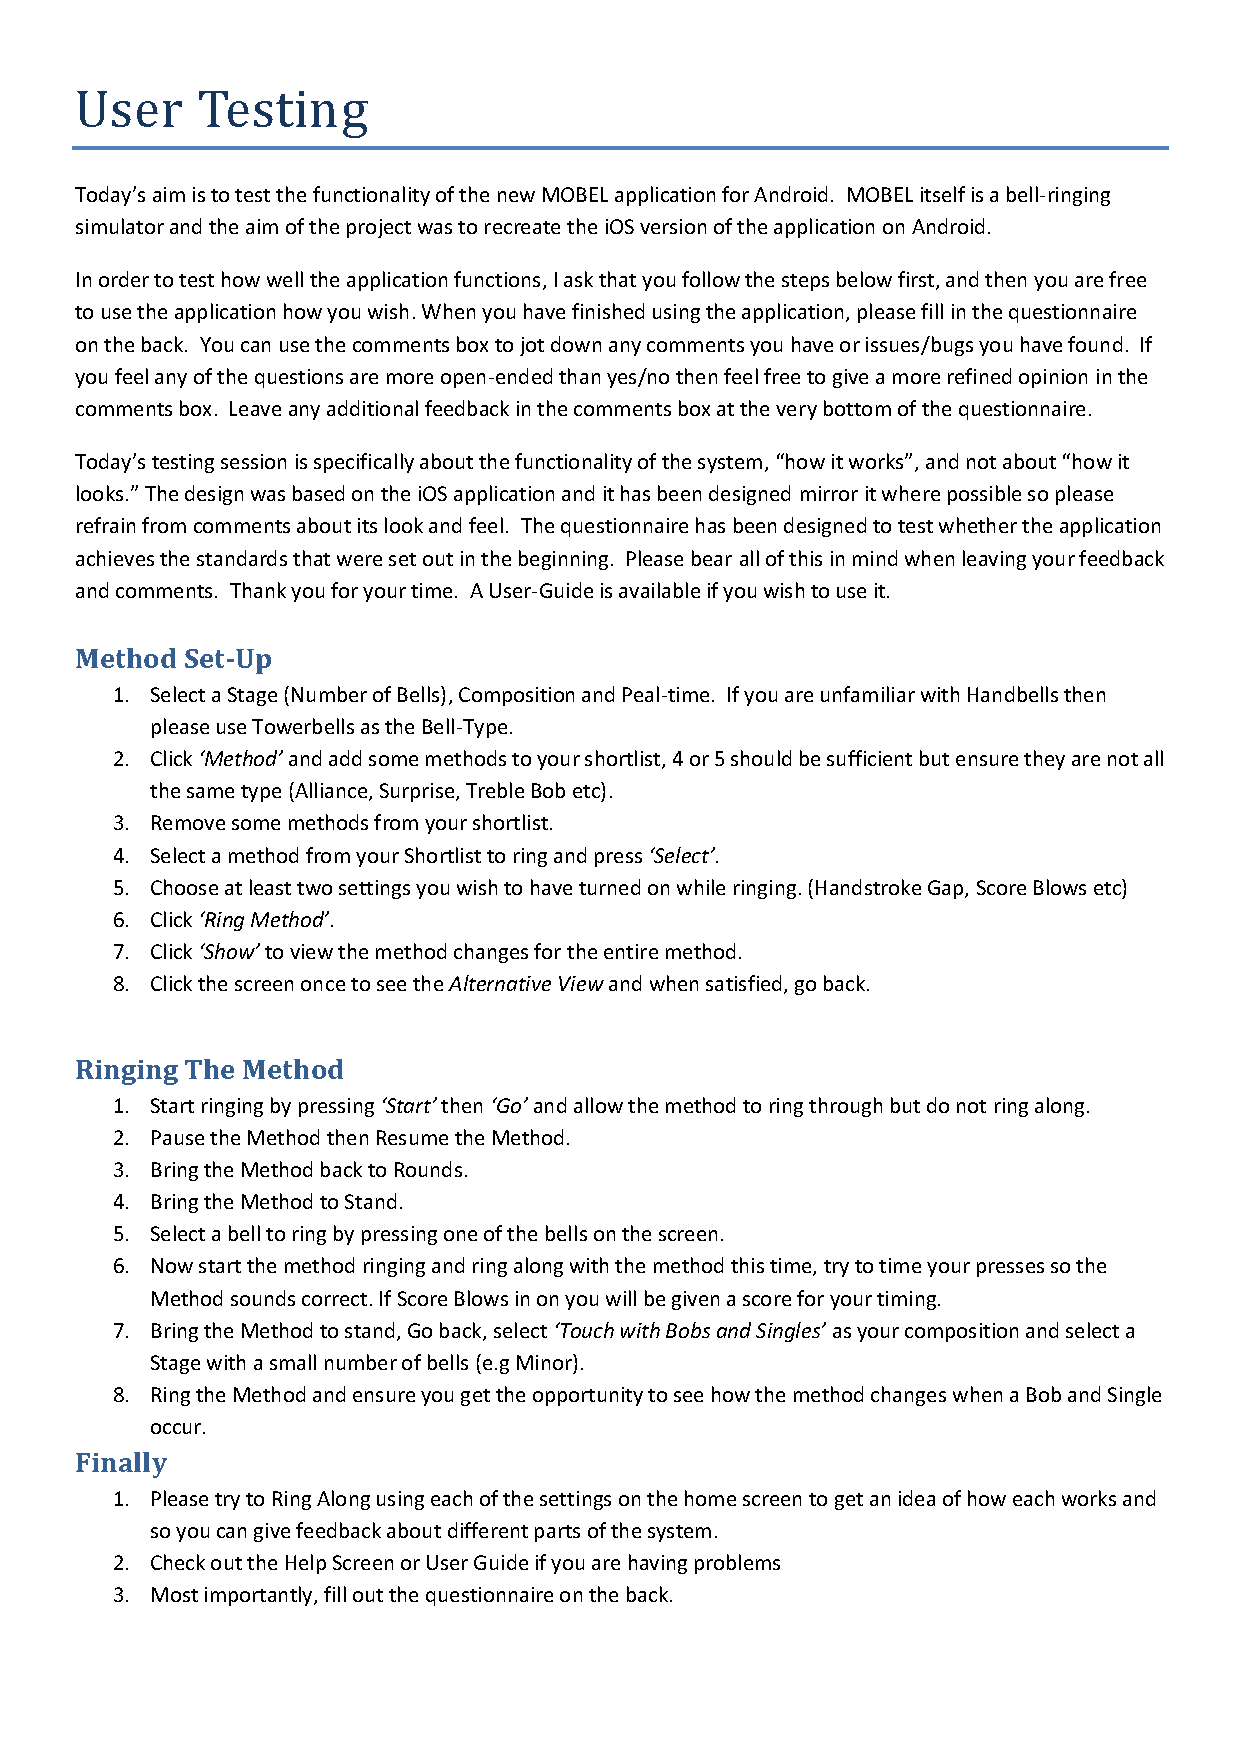
\includepdf[pages={1}]{UserTesting.pdf}
\includepdf[pages={2}]{UserTesting.pdf}

\chapter{Functional Requirements \& Testing Relationship}

\begin{tabular}{| p{2.5cm}| l | l | l | l |}
\hline
\textbf{Functional Requirement ID} &\textbf{Priority} & \textbf{Implemented} & \textbf{Related Test ID} & \textbf{Requirement Met}\\
\hline
\hline
FR-1 & Must Have & Yes & T1 & Yes\\
\hline
FR-2 & Must Have & Yes & T2 & Yes\\
\hline
FR-3 & Must Have & Yes & T3 & Yes\\
\hline
FR-4 & Must Have & Yes & T4 & Yes\\
\hline
FR-5 & Must Have & Yes & T20 & Yes\\
\hline
FR-6 & Must Have & Yes & T5 & Yes\\
\hline
FR-7 & Must Have & Yes & T6, T7 & Yes\\
\hline
FR-8 & Must Have & Yes & T8, T27, T28 & Yes\\
\hline
FR-9 & Must Have & Yes & T9 & Yes\\
\hline
FR-10 &Must Have & Yes & T10 & Yes\\
\hline
FR-11 &Must Have & Yes & T11, T17 & No\\
\hline
FR-12 & Must Have &Yes & T18, T19 & Yes\\
\hline
\hline
FR-13 & Should Have & Yes & T14, T15 & Yes\\
\hline
FR-14 & Should Have & Yes & T16, T18 & Yes\\
\hline
FR-15 & Should Have & Yes & T21 & Yes\\
\hline
FR-16 & Should Have & Yes & T22 & Yes\\
\hline
FR-17 & Should Have & Yes & T23 & Yes\\
\hline
FR-18 & Should Have & Yes & T24 & Yes\\
\hline
FR-19 & Should Have & Yes & T25 & Yes\\
\hline
FR-20 & Should Have & Yes & T26 & Yes\\
\hline
FR-21 & Should Have & Yes & T16 & Yes\\
\hline
FR-22 & Should Have & Yes & T5 & Yes\\
\hline
FR-23 & Should Have & Yes & T28 & Yes\\
\hline
FR-24 & Should Have & Yes & T29 & Yes\\
\hline
\hline
FR-25 & Could Have & No & - & No \\
\hline
FR-26 &Could Have & No & -& No \\
\hline
FR-27 &Could Have & No & - & No \\
\hline
FR-28 & Could Have &Yes & T13 & Yes\\
\hline
\hline
FR-29 &Would Have & No & - & No \\
\hline

\hline


\end{tabular}

\chapter{Generating Random Graphs}
\label{sec:randomGraph}
We generate Erd\'{o}s-R\"{e}nyi random graphs $G(n,p)$ where $n$ is the number of vertices and
each edge is included in the graph with probability $p$ independent from every other edge. It produces
a random graph in DIMACS format with vertices numbered 1 to $n$ inclusive. It can be run from the command line as follows to produce 
a clq file
\begin{verbatim}
      > java RandomGraph 100 0.9 > 100-90-00.clq
\end{verbatim}
\end{appendices}

%%%%%%%%%%%%%%%%%%%%
%   BIBLIOGRAPHY   %
%%%%%%%%%%%%%%%%%%%%

\bibliographystyle{plain}
\bibliography{bib}
http://ringing.org/main/pages/change-ringing
\end{document}
